\documentclass[11pt]{article}

\usepackage{float}
\usepackage{graphicx}
\usepackage{hyperref}
\hypersetup
{
    colorlinks=true,
    linkcolor=black,
    filecolor=blue,      
	urlcolor=blue,
	citecolor=black
}

\title{Machine Learning -- Homework 1}
\author{Andrea Gasparini \\ \texttt{1813486}}
\date{November 2020}

\begin{document}

	\maketitle

	\tableofcontents	

	\newpage



	\section{Introduction}
	The task of this Homework was to build a \textit{multiclass classifier} to
	determine whether an assembly function is an \textbf{encryption}, \textbf{math},
	\textbf{string manipulation} or \textbf{sorting} function.
	Formally, the task was to aproximate a mapping function:
	\begin{equation} \label{eq:mapping-function}
		f : X_{bin} \rightarrow \{ encryption, math, string, sort \}		
	\end{equation}
	where $ X_{bin} $ is an assembly set of instructions that can be classified
	in one of the target classes of the $ f $ function's right-hand side.
	To be more precise, since we have to define a features list to train a
	Machine Learning model, $ X_{bin} $ is a list of measurable properties
	extracted from the dataset after a feature extraction procedure
	(\autoref{subsec:feature-extraction}).



	\section{The Dataset}
	The dataset used to train the model was provided in two versions:
	\begin{itemize}
		\item With 14397 assembly functions, containing duplicates
		\item With 6073 assembly functions, without duplicates
	\end{itemize}
	As we can see in \autoref{fig:datasetnodup}, removing the duplicates creates
	an unbalanced dataset and this can lead to problems in predicting the minority
	class. An oversampling procedure has probably been applied to obtain
	the dataset with duplicates and solve the unbalancing problem.
	Training a model with both versions of the dataset allowed to evaluate the
	differences with some metrics and then choose the best one.

	\begin{figure}[ht]
		\centering
		\begin{minipage}{.5\textwidth}
		  \centering
		  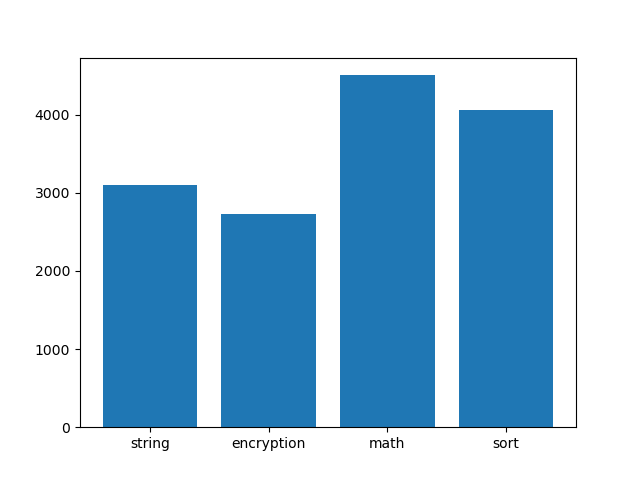
\includegraphics[width=\linewidth]{assets/dataset.png}
		  \caption{Dataset with duplicates}
		  \label{fig:dataset}
		\end{minipage}%
		\begin{minipage}{.5\textwidth}
		  \centering
		  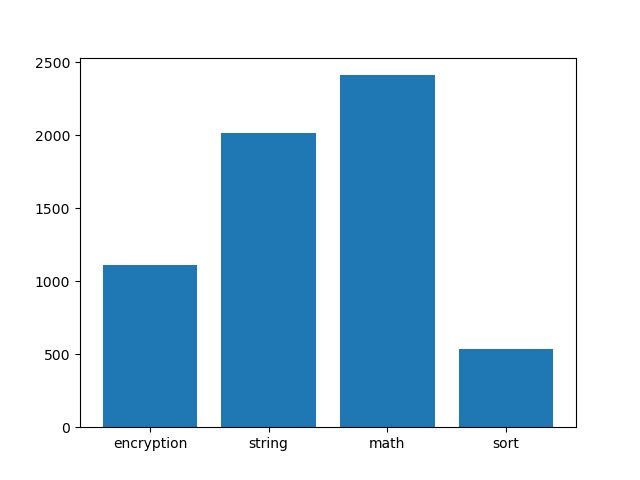
\includegraphics[width=\linewidth]{assets/datasetnodup.png}
		  \caption{Dataset without duplicates}
		  \label{fig:datasetnodup}
		\end{minipage}
	\end{figure}


	\subsection{Undersampling procedure}
	Another dataset could be obtained applying an undersampling procedure on the
	one without duplicates. 
	In other words, removing some entries of the majority classes to obtain a
	balanced distribution of all classes.
	The problem with this approach is in the size of the original dataset and of
	the minority class (\textit{sort}), the process could lead to loss of valuable
	information and to a too small dataset. The idea was then discarded.


	\subsection{Data format}
	Each entry of the dataset, provided as a \texttt{JSON}, represent an assembly
	function and contains:
	\begin{itemize}
		\item The label of the function, that is one of the target classes defined
		in \autoref{eq:mapping-function} (\textit{math}, \textit{sort}, \textit{encryption} or \textit{string})
		\item The linear list of his assembly instructions
		\item The control flow graph (CFG), econded as a NetworkX graph
	\end{itemize}



	\section{Preprocessing and feature extraction} \label{subsec:feature-extraction}
	Since the assembly instructions were encoded as lists of strings, a first
	approach I tried was to solve the task as a standard \textit{text classification
	problem}. In this way the features list for the model contained the 
	occurences' number of every "word" in the assembly functions.
	The main problem in this case was caused by the lack of a \textit{stop words}
	set. In fact, in a \textit{text classification problem} we should always
	specify which words don't have to be considered because of their common use
	in the language (such as \textit{the}, \textit{is}, \textit{which}, etc) and
	focus on the important words instead.
	For example counting the occurences of words representing registers wasn't
	necessary and could lead to wrong predictions.
	Then I changed the approach and thought of a better way to extract some specific
	characteristics from the dataset to train the model.

	\subsection{Characteristics of the target classes} \label{subsec:target-classes}
	For every target class we had some hints about its common characteristics:
	\begin{itemize}
		\item \textit{encryption}: contains a lot of nested \texttt{for} and
		\texttt{if} (i.e. a complex CFG), uses a lot of \texttt{xor}, shifts and
		bitwise operations, and is extremely long
		\item \textit{sort}: contains one or two nested \texttt{for} and some
		helper functions, uses compare and moves operations
		\item \textit{math}: uses a lot of arithmetic operations and special
		registers \texttt{xmm*} for floating point instructions
		\item \textit{string}: uses a lot of comparisons and swap of memory locations
	\end{itemize}
	The point was to take advantage of these characteristics to map the dataset's
	entries to features lists that could be used to train a model.
	Every entry in the dataset has been processed and mapped in a list with the
	following 9 features:
	\begin{itemize}
		\item \textit{graph\_nodes}: is the number of nodes in the CFG, where each
		node represents a \textit{basic block}, i.e. a straight-line piece of code
		without any jumps or jump targets
		\item \textit{graph\_diam}: is the maximum diameter value of the CFG's
		strongly connected components, where the diameter of a component represents
		the maximum distance between its pair of vertices
		\item \textit{mov}: is the number of \texttt{mov} instrunctions in the function
		\item \textit{bitwise}: is the number of bitwise instrunctions in the function
		\item \textit{xmm}: is the number of \texttt{xmm} registers in the function
		\item \textit{arithm}: is the number of arithmetic instrunctions in the function
		\item \textit{cmp}: is the number of \texttt{cmp} instrunctions in the function
		\item \textit{shift}: is the number of shift instrunctions in the function
		\item \textit{calls}: is the number of calls instrunctions in the function
	\end{itemize}	



	\section{Evaluation}
	In order to evaluate a solution based on a features list it's necessary to
	train some models and compare the performances according to some metrics.

	The comparisons in this report are based on the results obtained from two
	models: \textbf{Decision Tree} and \textbf{Support Vector Machine}.
	I used different metrics to evaluate the correctness of these models, like
	plotting the \textit{confusion matrices} and comparing \textit{precision},
	\textit{recall} and \textit{f1-score}.
	Another metric taken in consideration was the way of splitting the dataset.
	In fact the standard way is to reserve $\frac{2}{3}$ for the training
	and $\frac{1}{3}$ for the test. Decreasing the first one and therefore
	increasing the second one could get worse performances, but whether we still
	get acceptable results the approach is probably working well.

	\paragraph{Precision}
	With \textit{precision}, for a certain class $x$, we indicate the percentage of correctly
	predicted instances among all the instances predicted as $x$:
	\[
		\frac{TP}{TP + FP}
	\]
	where TP represents the correctly classified instances count and FP the wrongly
	classified as $x$ count.

	\paragraph{Recall}
	With \textit{recall}, for a certain class $x$, we indicate the percentage of correctly
	predicted instances among all the really $x$:
	\[
		\frac{TP}{TP + FN}
	\]
	where FN represents the instances count of $x$ wrongly classified in another class.

	\paragraph{F1 score}
	The \textit{F1 score} is the harmonic mean between \textit{precision} and \textit{recall}
	\[
		\frac{2 \cdot precision \cdot recall}{precision + recall}
	\]

	\paragraph{Confusion Matrix}
	A confusion matrix is an easy way to visualize the performance of a learning algorithm. 
	Each row of the matrix represents the number of instances (or the percentage
	if it's normalized) in the true class while each column represents the instances in
	a predicted class.
	All correct predictions are located in the diagonal of the table, which elements
	represent the \textit{recall} values, so it is easy to visually inspect the table
	for prediction errors, as they will be represented by values outside the diagonal.

	\subsection{Comparisons}
	The following comparisons shows the \textit{confusions matrices} resulting
	of the two models' training on the dataset with duplicates (with-dup), and
	on the dataset without duplicates (no-dup).
	Comparisons have been made with a test size of 33\% and of 66\% to check if
	the accuracy consequently decreases or the results remain good.
	
	\subsubsection{Decision Tree}
	With this model the first impression with the final features list
	was to have an overfitting since the performance (\autoref{fig:dt-with-dup-33})
	seemed to be too high.
	An increase in the test size did not decrease the performance and this led me
	to reconsider the assumption of overfitting.
	The dataset without duplicates had a predictable result since the \textit{sort}
	class was the minority. 

	\begin{figure}[H]
		\centering
		\begin{minipage}{.5\textwidth}
		  \centering
		  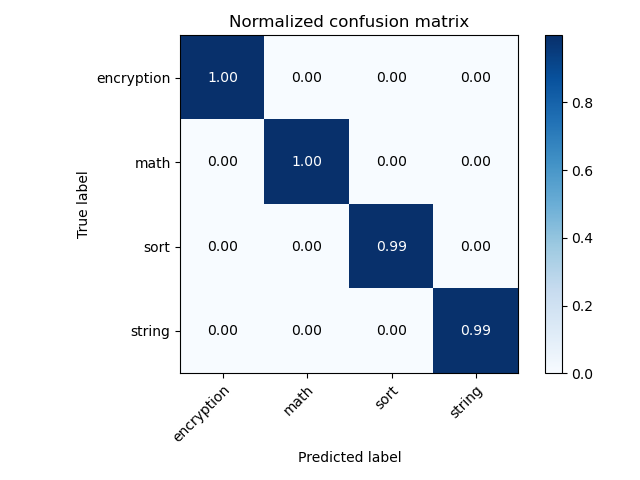
\includegraphics[width=\linewidth]{assets/tree_dup_0.333.png}
		  \caption{DT with-dup -- test 33\%}
		  \label{fig:dt-with-dup-33}
		\end{minipage}%
		\begin{minipage}{.5\textwidth}
		  \centering
		  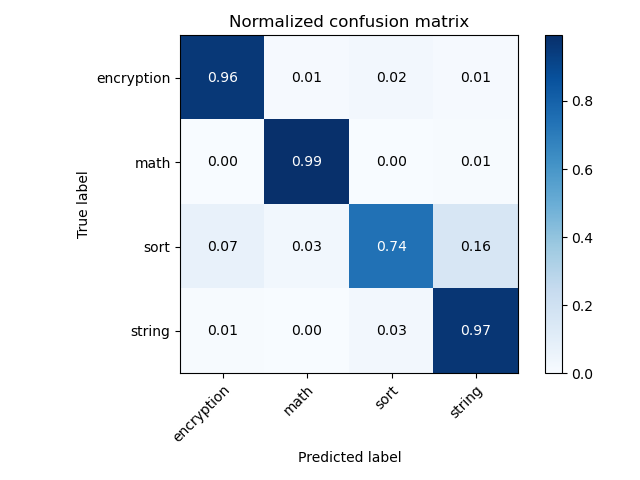
\includegraphics[width=\linewidth]{assets/tree_nodup_0.333.png}
		  \caption{DT no-dup -- test 33\%}
		\end{minipage}
	\end{figure}

	\begin{figure}[H]
		\centering
		\begin{minipage}{.5\textwidth}
		  \centering
		  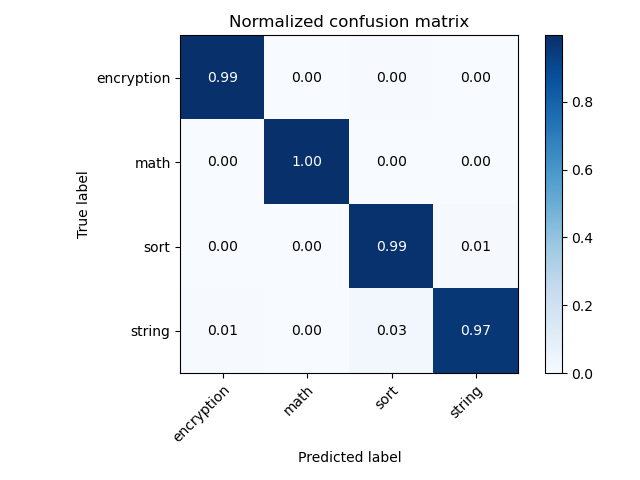
\includegraphics[width=\linewidth]{assets/tree_dup_0.66.png}
		  \caption{DT with-dup -- test 66\%}
		\end{minipage}%
		\begin{minipage}{.5\textwidth}
		  \centering
		  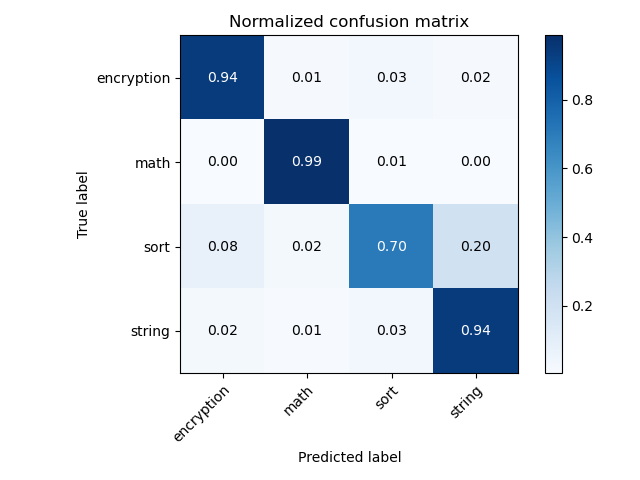
\includegraphics[width=\linewidth]{assets/tree_nodup_0.66.png}
		  \caption{DT no-dup -- test 66\%}
		\end{minipage}
	\end{figure}

	\subsubsection{Support Vector Machine}
	In this case the model needed to be configured with a kernel and a parameter
	$C$, that have been set after some tests respectively as \texttt{linear} and
	1 to have the best trade-off in performance and training time.
	Compared to the Decision Tree, SVM had a little worse performance, but still
	really good.
	The model performed better without the duplicates, with an increase in the
	Recall for every target class except for \textit{sort}, because it was the
	minority class in the unbalanced dataset.
	\begin{figure}[H]
		\centering
		\begin{minipage}{.5\textwidth}
		  \centering
		  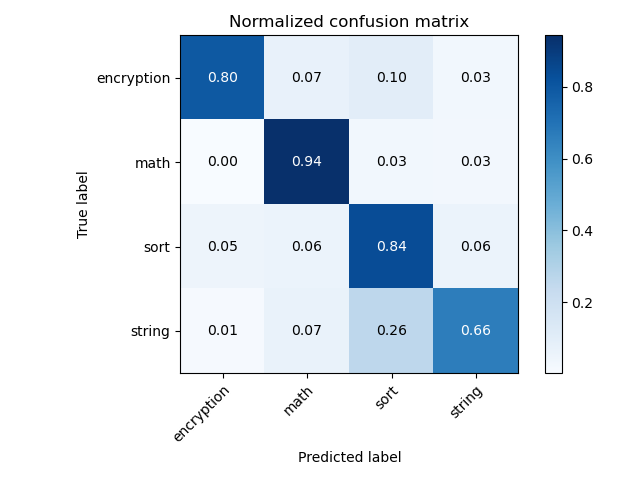
\includegraphics[width=\linewidth]{assets/svc_dup_0.333.png}
		  \caption{SVM with-dup -- test 33\%}
		\end{minipage}%
		\begin{minipage}{.5\textwidth}
		  \centering
		  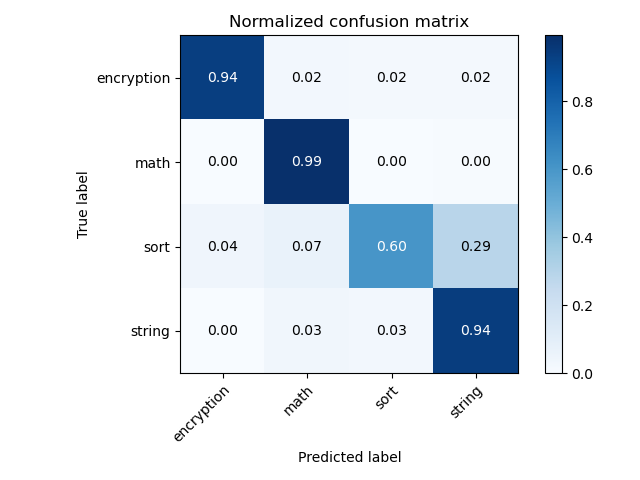
\includegraphics[width=\linewidth]{assets/svc_nodup_0.333.png}
		  \caption{SVM no-dup -- test 33\%}
		\end{minipage}
	\end{figure}

	\begin{figure}[H]
		\centering
		\begin{minipage}{.5\textwidth}
		  \centering
		  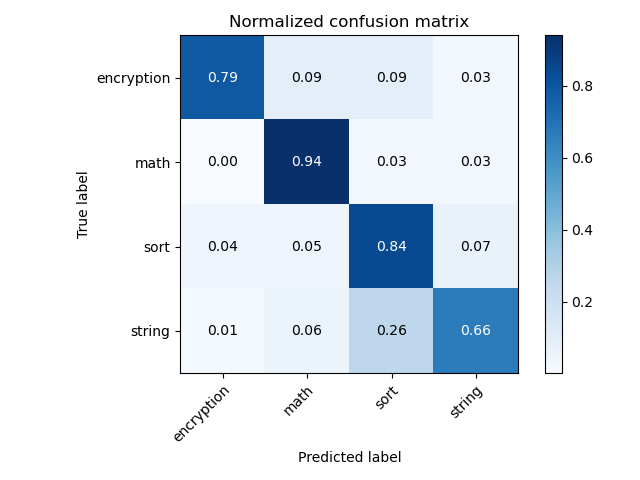
\includegraphics[width=\linewidth]{assets/svc_dup_0.66.png}
		  \caption{SVM with-dup -- test 66\%}
		\end{minipage}%
		\begin{minipage}{.5\textwidth}
		  \centering
		  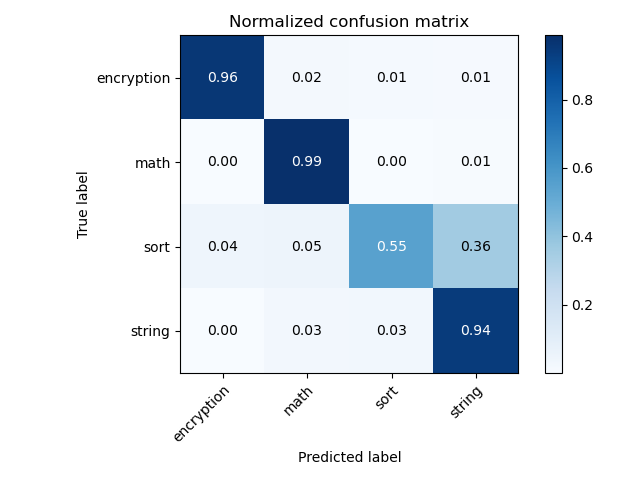
\includegraphics[width=\linewidth]{assets/svc_nodup_0.66.png}
		  \caption{SVM no-dup -- test 66\%}
		\end{minipage}
	\end{figure}	



	\section{Conclusions}
	The final features list defined in \autoref{subsec:target-classes} was obtained
	after some tests with less features and more than two models. The results showed
	seemed to be the best ones and a big increase in the performance was granted
	by the use of the CFG features (\textit{graph\_nodes} and \textit{graph\_diam}).
	For example by replacing \textit{graph\_nodes} with an apparently similar feature
	that is the number of assembly instructions we get 10\% worse performance.
	
	We can tell from the previous comparisons that Decision Tree obtains the
	best results with both datasets. The first impression was to have an overfitting
	since a Recall near to 0.99 seemed to be too high, but the results were still
	good with the second dataset (no-dup) and also with an increased test size,
	i.e. a decreased training size (that I thought should led to worse results).
	Another reason to prefer Decision Tree was the training time, that was always
	better than tested configurations of SVM without having worse performances.

	In both cases the bigger problem was in the misclassification of \textit{sort}
	and \textit{string} functions, in fact both DT and SVM could classify a \textit{sort}
	function as a \textit{string} one because of the low number of instances.
	Incrementing the number of \textit{sort} instances in dataset without
	adding duplicates would certainly improve the performances for these cases,
	but produce this new data would require a lot of effort.
\end{document}